% Please do not change the document class
\documentclass{scrartcl}

% Please do not change these packages
\usepackage[hidelinks]{hyperref}
\usepackage[none]{hyphenat}
\usepackage{setspace}
\usepackage{graphicx}
\graphicspath{ {G:/GitHubGames/comp110-architecture-essay/Pictures/} }
	
\doublespace

% You may add additional packages here
\usepackage{amsmath}

% Please include a clear, concise, and descriptive title
\title{Implementation of PCG: Three Examples But Which Is The Most Practical?}

% Please do not change the subtitle
\subtitle{COMP110 - Computer Architecture Essay}

% Please put your student number in the author field
\author{1506530}

\begin{document}

\maketitle

\abstract{Procedural content generation (PCG) has been used in games for decades now. It is an ever evolving method for creating emersive and reliable game that players can enjoy. This paper will provide three distinct methods for implementing PCG in a 2D platfrom game. They will be of an increasing implementation ease, starting from a relatively simple algorithm that is used to enhance the difficulty of a game. Then moving on to one that uses an already existing game to randomize its levels. Finally creating a complete new game based on PCG.}

\section{Introduction}

Procedural content generation (PCG) is one of many methods used today to create and design levels, particularity 2D platformers. PCG not only creates a new experience for the player with each playthrough, but also when done correctly can keep development costs down, by removing the need for extra level designers\cite{walaa}. The only real issue with PCG is which one to choose, with the variety of algorithms that are available it can be daunting to decide on which direction to go. So with PCG its important to have a clear idea of the task you want to accomplish as this will clearly define which algorithm would be the best for that game. With this in mind this paper contains three different algorithms that could be used in a 2D Platform game. 

\subsection{Motivation}
The three examples used are to be discussed on which algorithm would be the easiest to implement while still being the most efficient. They are as follows:
\newline 
In section 2: An Iterative Content Adaptation Algorithm (ICA) used to enhance difficulty of a game\cite{fausto}.
\newline
Section 2.1: Genetic Algorithm (GA) used alongside an Agent-based Digger Algorithm to use and add assets to an established game\cite{walaa}.
\newline
Section 2.2: An Algorithm used alongside the Launchpad to create a whole new game\cite{web}.
\newline
In section 3: A comparison of efficiency will be drawn based on their respective results.
\newline
More detailed information can be found here \cite{fausto,walaa,web} respectively. Aa brief a description as possible for each algorithm and how they work are presented in the following sections. Looking at ease of implementation the obvious choice would be the ICA due to its simplicity and ease of use on more than one game, more on this in section 2.

\section{Iterative Content Algorithm (ICA)}

The First Algorithm that is looked at is perhaps the easiest to implement, as it uses a graph overlay of a generated map to populate the map with objects and obstacles. A graph is drawn form the geometry of each level to create something similar to the graph in Fig.1 Prince of Persia was used for these examples \cite{fausto}.
\newline
\newline
\begin{figure}[h]
	\centering
	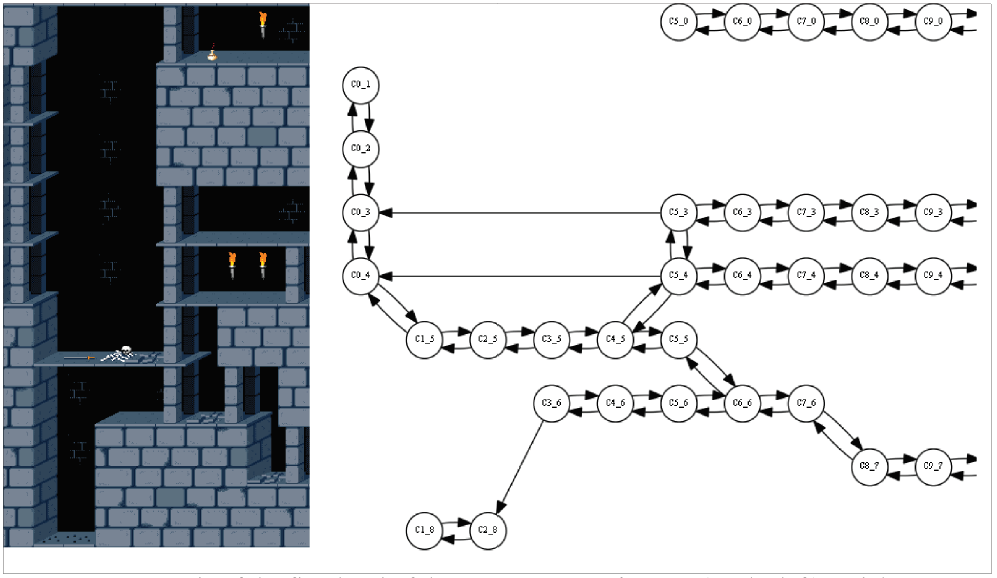
\includegraphics[width=0.7\linewidth]{Fig1}
	\caption{ - A Sample of the first level of the game \textit{Prince of Persia} (on the left) and the graph (on the right)}.
	\label{Fig1}
\end{figure}\cite{fausto}


As you can see there is quite a bit of information here which requires more computational effort from the algorithm than is required. So the graph needs to be compressed as to reduce the amount of vertices and edges there are. For example the if a vertex is connected directly to another vertex it will stay, if not then its removed to produce a graph like Fig.2\cite{fausto}.
\newline
\newline
\newline
\newline
\newline
\newline
\begin{figure}[h]
	\centering
	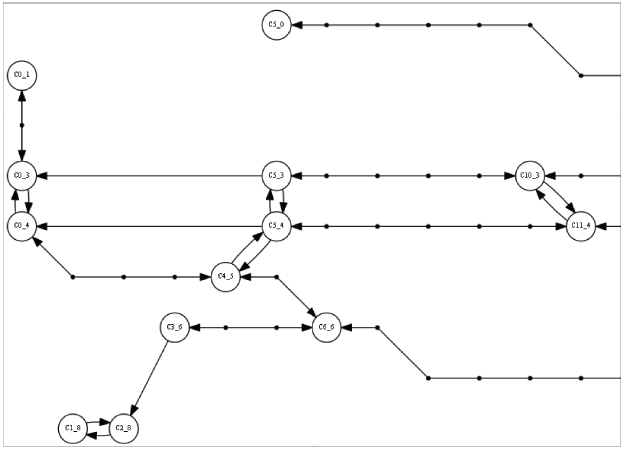
\includegraphics[width=0.7\linewidth]{Fig2}
	\caption{ - Example of a compressed graph. The compressed nodes are marked with dots}.
	\label{Fig2}
\end{figure}\cite{fausto}


As can be derived from these there is a significant difference. The ICA will then calculate the shortest/longest/alternative routes to the end of each level with the addition of dead-ends and a no way back path. This is gathered into a tree presenting all the information in a more readable manner alongside the graph Fig.3\cite{fausto}.
\newline
\newline
\newline
\begin{figure}[h]
	\centering
	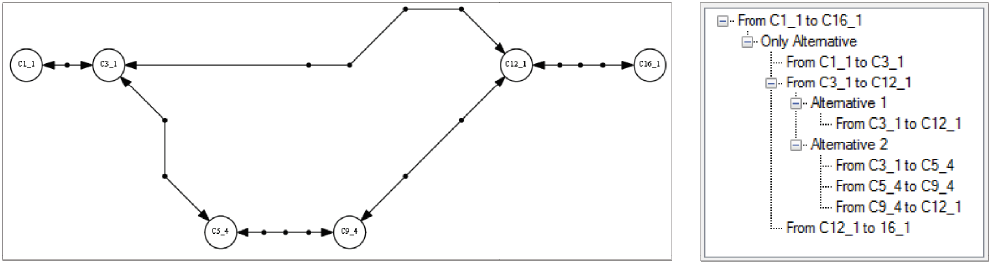
\includegraphics[width=0.7\linewidth]{Fig3}
	\caption{ - Example of a graph (on the left) and the corresponding tree (on the right)}.
	\label{Fig3}
\end{figure}\cite{fausto}


From this, its is overlayed onto a platform level Fig.4.Then with difficulty applied, in Fig.5 a difficulty level of 100 was tested\cite{fausto}.
\newline
\newline
\newline
\begin{figure}[h]
	\centering
	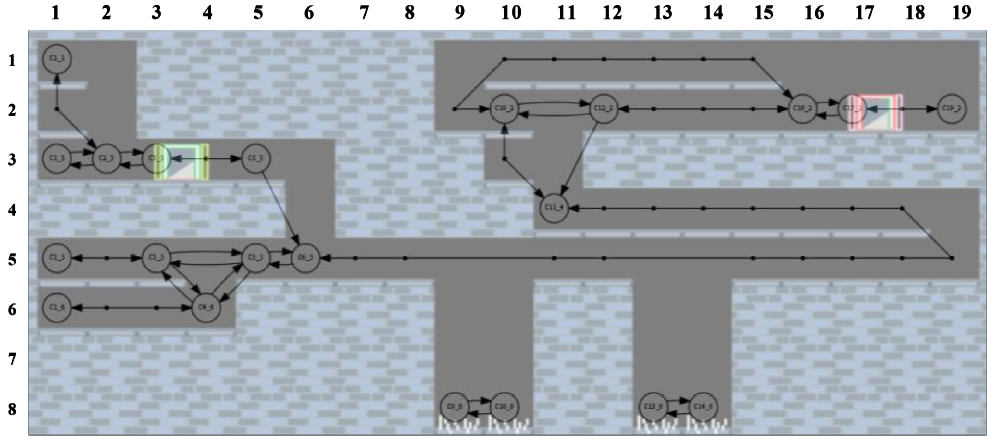
\includegraphics[width=0.7\linewidth]{Fig4}
	\caption{ - The Graph generated for the example level}.
	\label{Fig4}
	\centering
	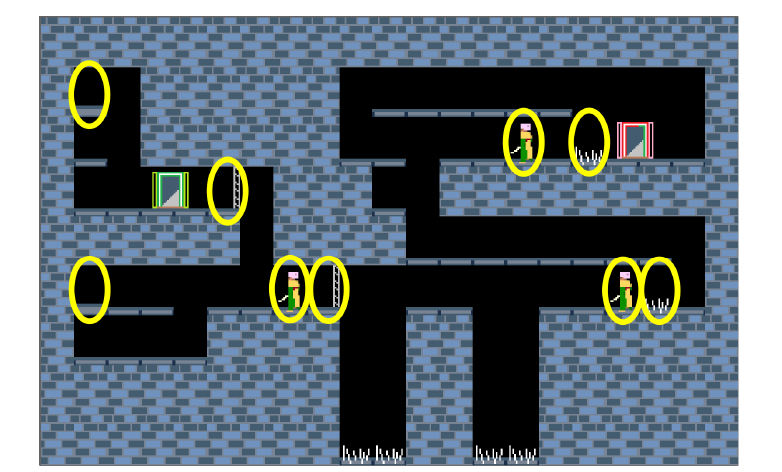
\includegraphics[width=0.7\linewidth]{Fig5}
	\caption{ - Example of the level after the algorithm has been applied to \textit{Prince of Persia}}.
	\label{Fig5}
\end{figure}\cite{fausto}


From Fig.4 its can be seen that the algorithm also used the dead-ends to apply another challenge in the from of switches to remove the obstacles from the path. This method can also be applied to other platform based games as can be seen in Fig.6.7. This can be really useful for cutting costs in development as it removes the need for object placement in games. Although the developer will still need to create the levels themselves, they would not need to be populated\cite{fausto}.
\newline
\newline
\begin{figure}[h]
	\centering
	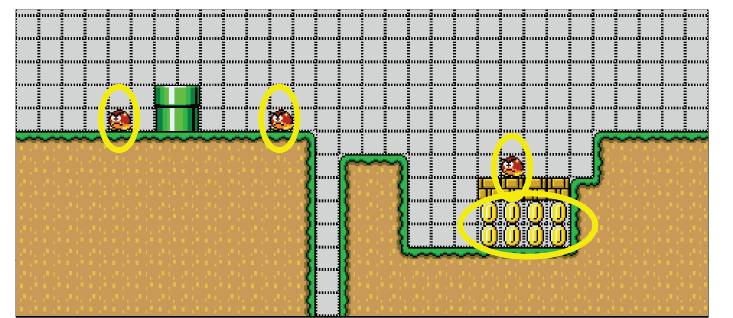
\includegraphics[width=0.7\linewidth]{Fig6}
	\caption{ - Example of the level after the algorithm has been applied to \textit{Infinite Mario Bros.}}.
	\label{Fig6}
	\centering
	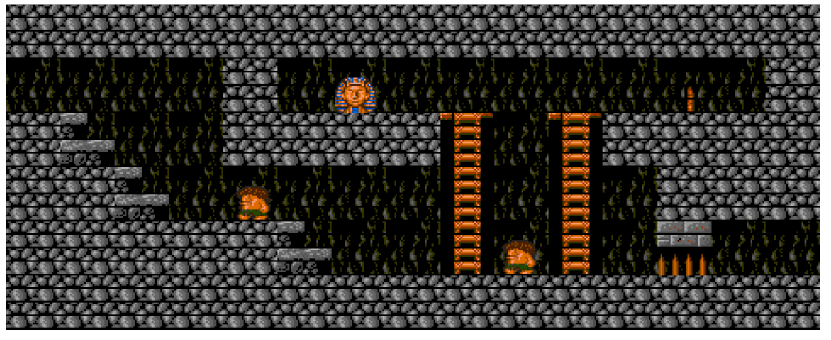
\includegraphics[width=0.7\linewidth]{Fig7}
	\caption{ -Example of the level after the algorithm has been applied to \textit{XRick}}.
	\label{Fig7}
\end{figure}\cite{fausto}


\subsection{Genetic Algorithm (GA)}

Genetic Algorithm (GA) is a search heuristic that will mimic the natural selection process, a taxonomy of a evolutionary algorithm that runs through hundreds of evolutions to determine the most optimized method for the task at hand\cite{tax}. Using this algorithm, Infispel, an adaptation of the famous platform game Spelunky is a good example where this is used. A Genetic Algorithm (GA) along with graphs of the rooms and the paths connecting them is used to populate the levels with items and objects. While a agent-based Digger algorithm is used for the rooms structure depending on the difficulty selected Fig.8. Primarily for map building in a first-person shooter games the digger algorithm can provide a platformer game with interesting level builds Fig.8. \cite{walaa}. The way in which the digger creates a level is its placed in one of the 16 rooms and is set of in a random direction, assigning each cell a value of 1(on) or 0(off). The digger will repeat this for a total of 35 moves, walls are then dug where necessary for room connection, then repeated again for the 16 rooms.  
\newline
\begin{figure}[h]
	\centering
	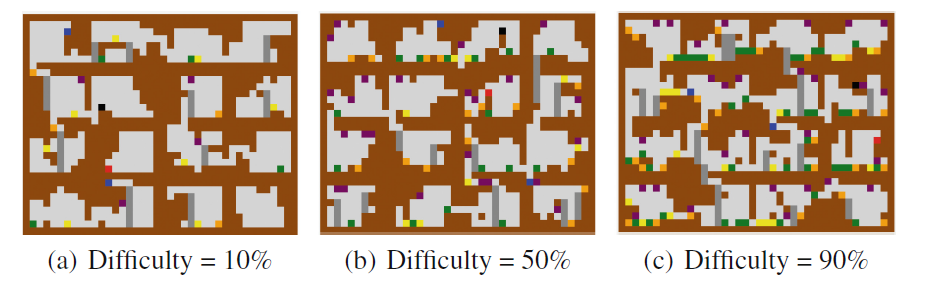
\includegraphics[width=0.7\linewidth]{Fig8}
	\caption{ - Three Examples of the digger outcome with increasing difficulty}.
	\label{Fig8}
\end{figure}\cite{walaa}

Through this method a developer could create a PCG game based only on these two Algorithms, but they would require quite a bit of modification before implementation unlike the ICA\cite{walaa,fausto}.

\subsection{Endless Web (EW)}

The last and biggest method would be using the Launchpad along with a PCG algorithm to create a game that continuously builds the game depending on your play style\cite{web}. With EW the approach taken was to use the Launchpad as the primary PCG source then extensively modify it to suit their needs. Fig.9 shows the capabilities of the end product.

\begin{figure}[h]
	\centering
	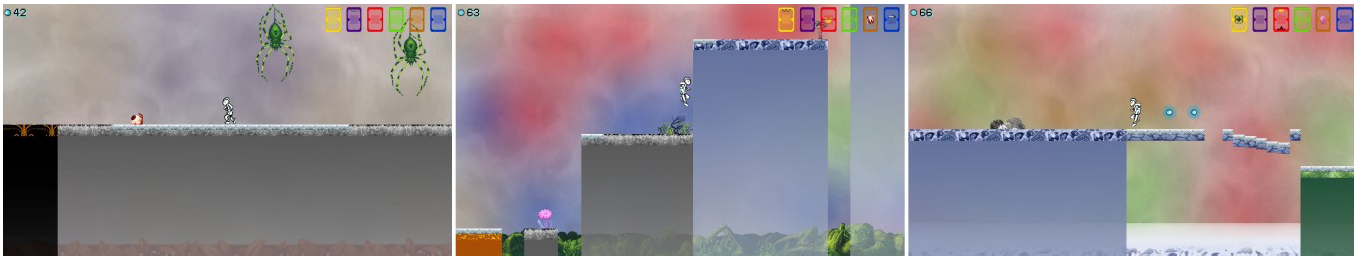
\includegraphics[width=0.7\linewidth]{Fig9}
	\caption{ - Three different scenarios that can come from Endless Web}.
	\label{Fig9}
\end{figure}\cite{web}

The game is dependant on the way you tune the world around you, by using different \textit(Tuning Portals) and the proximity to friendly NPC's the world around you will automatically generate and change\cite{web}. The development of such a PCG game would require a great deal of time and cost, for a small indie company it would be impractical to use such a method to create a game.

\section{Recommendation}

Through the Evidence provided in the whole section 2, the Iterative Content Algorithm (ICA) would be the strongest to use for a small indie company. As provided by section 2 the ICA is the easiest most practical method to implement PCG. It can support a wide variety of platfrom games with little to no modification\cite{fausto}. While the other two methods would require stronger modifications and commitment to achieve\cite{walaa,web}

\section{Conclusion}

Although further research is needed on all three methods presented here, it is clear that PCG is still evolving in many directions. From small item placement as seen with the ICA to churning out an entire game as you play as with The Endless Web. From this paper it is hoped that the reader can take away a fair and basic understanding of just a few ways which PCG can be done. Along with a good idea of which method would be useful when creating a game for themselves. A further question that could be asked is could these three methods be combined to create a new method of PCG. This would require further research into them for any feasible argument to be made.

\bibliographystyle{ieeetr}
\bibliography{comp110_architecture}

\end{document}
